\chapter{Le modifiche al SIMIOR}
Per accomodare le nuove funzionalità è stato necessario fare delle modifiche strutturali al SIMIOR, spaziando dal database a classi di gestione dei dati interne al front-end del progetto.
\section{Modifiche strutturali}\label{modifiche_strutturali}
Le modifiche fatte si possono raggruppare in tre punti:
\begin{itemize}
	\item Database
	\item Archivio Statico
	\item Front-End
\end{itemize}
Oltre al database che contiene i dati creati dagli utenti, il SIMIOR possiede dei dati "statici" che raramente richiedono una modifica, un esempio di questi dati sono i codici degli antibiotici definiti dal sistema ATC/DDD (Anatomical Therapeutic Chemical/Defined Daily Dose) o i codici dei microorganismi definiti dall'Istituto Superiore di Sanità.
Quando viene effettuato un inserimento di un antibiogramma (sia tramite la nuova funzionalità sia manualmente) il sistema effettua una ricerca in questo archivio statico per estrarre il codice relativo al microrganismo/antibiotico, ma inizialmente questi nomi erano in lingua inglese (sempre seguendo il sistema di origine dei dati) causando il fallimento dell'estrazione. Per ovviare a questo problema si è prima provveduto ad aggiornare l'archivio con la versione italiana e in secondo luogo aggiungendo la possibilità di avere un valore alternativo per casi particolari verificati in alcuni referti.
Che altro ho cambiato?
\newpage
\section{Implementazione FrontEnd}
L'utente può utilizzare la funzionalità recandosi nella sezione \textit{infezione, contaminazione o colonizzazione} di un qualsiasi ricovero, dove troverà una scheda contenente l'essenziale per poter allegare un referto e procedere con il caricamento.
Ogni sezione è stata progettata per essere semplice e analoga ad altre parti del progetto per evitare confusione da parte dell'utilizzatore finale che è già abituato ai meccanismi del sistema. Infatti la schermata dei risultati ha lo stesso aspetto dell'inserimento manuale dell'antibiogramma (una funzione di base del SIMIOR) con qualche aggiunta resa necessaria.
\subsection{Localizzazione della funzionalità}
\begin{figure}[h!]
	\centering
	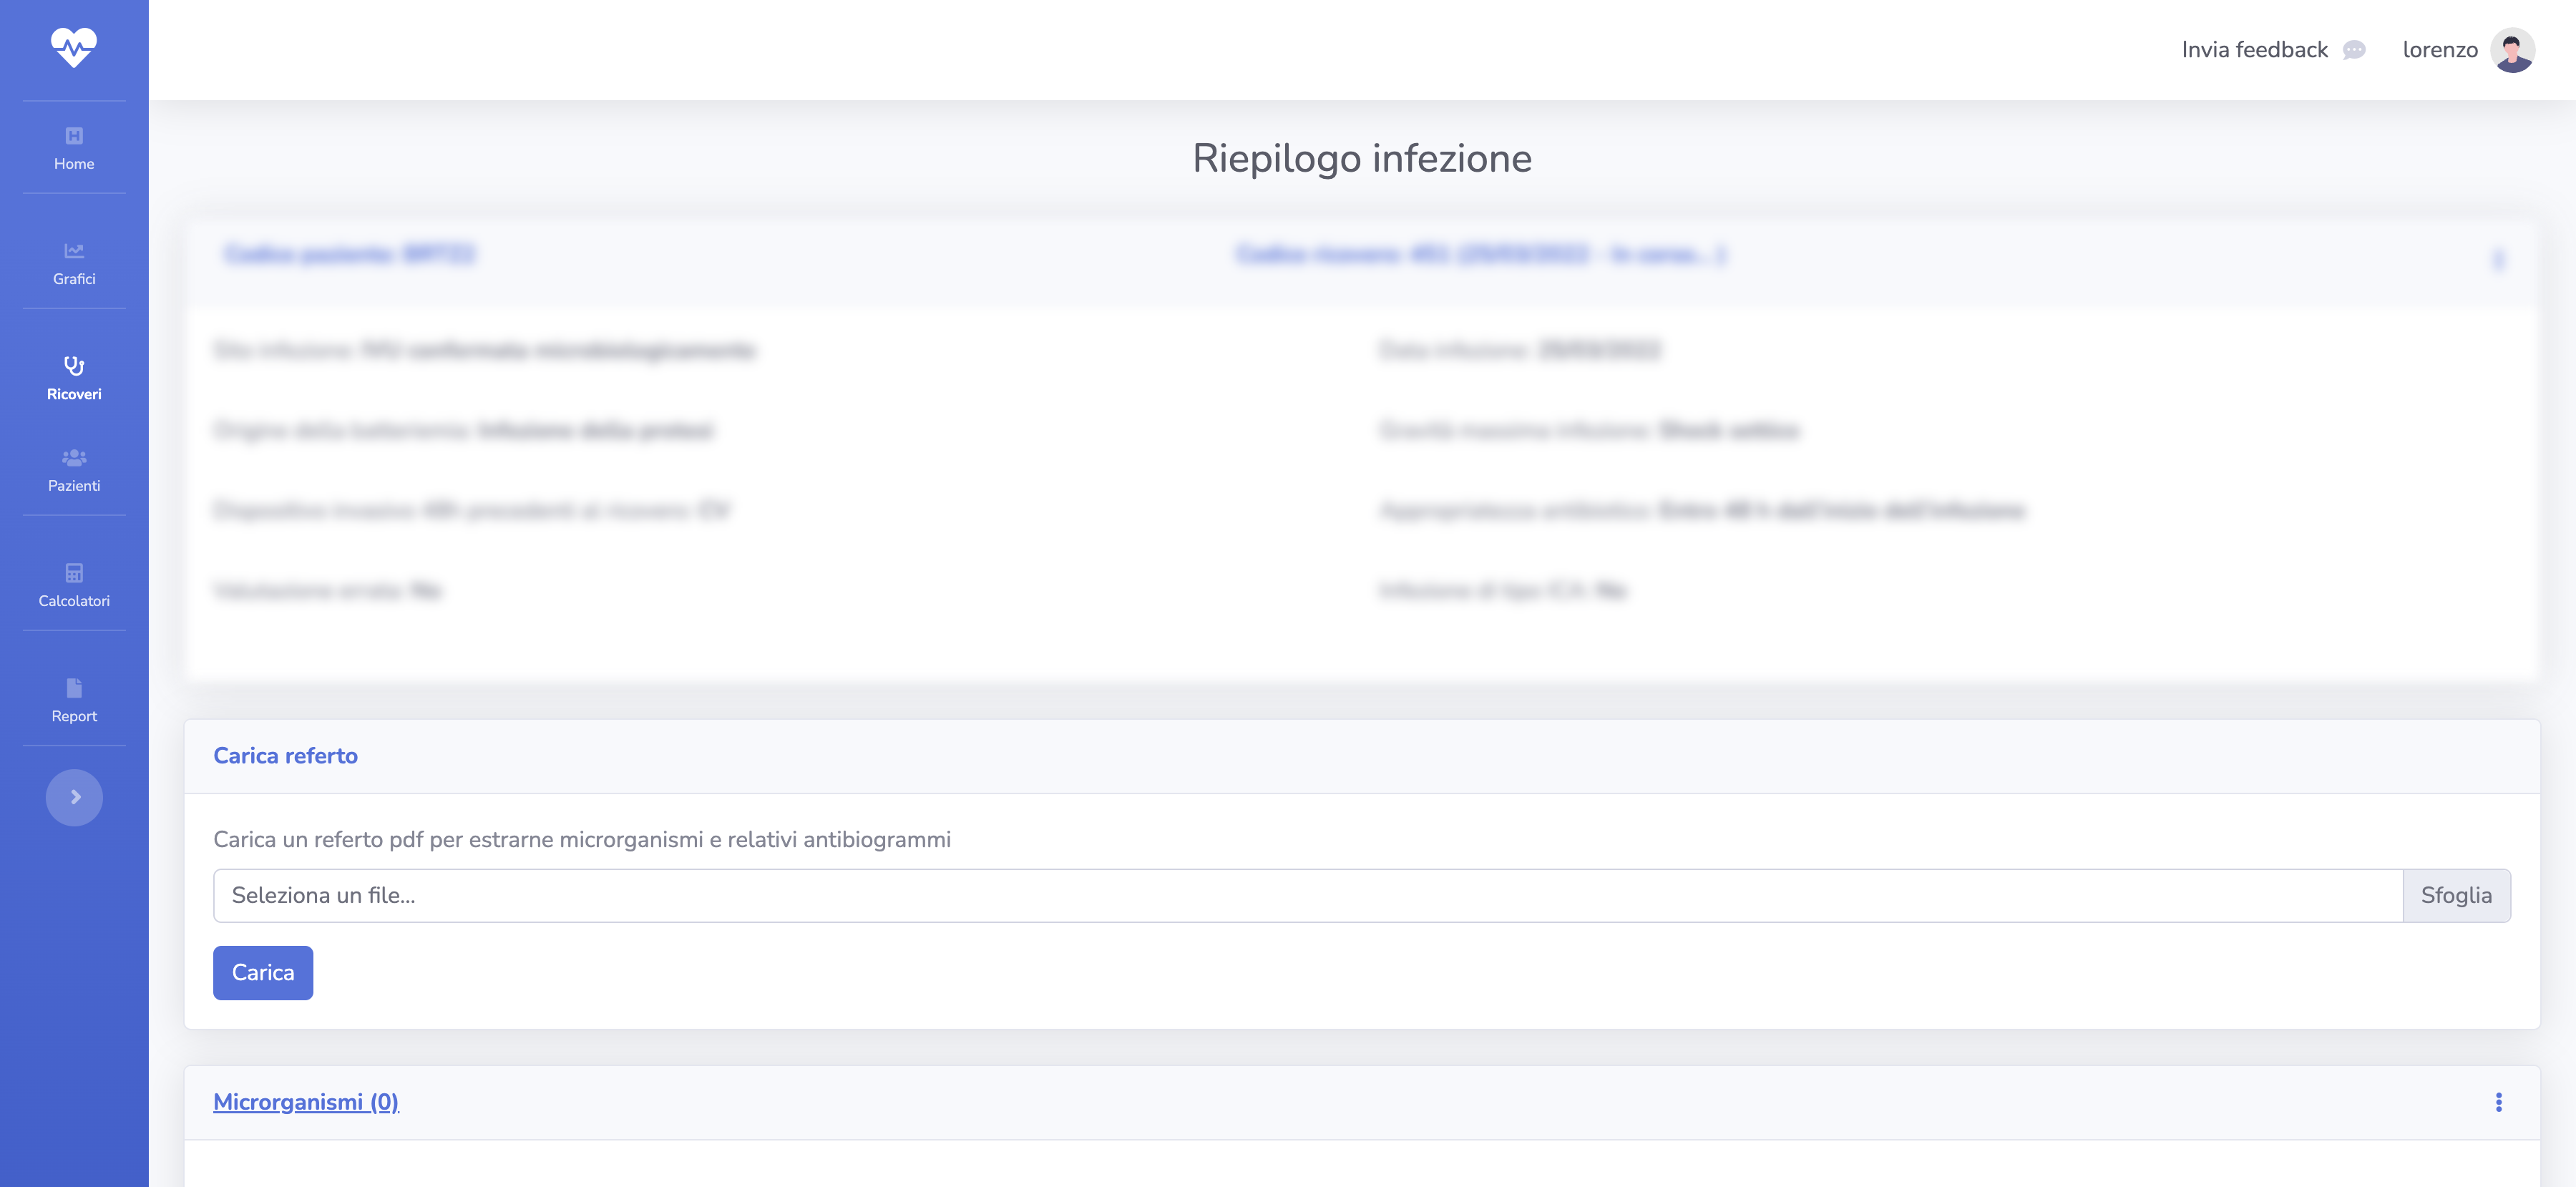
\includegraphics[width=.99\columnwidth]{images/feature_location.png}
	\caption{\textit{Scheda upload documento}}
	\label{fig:feature_location}
\end{figure}
La pressione del tasto \textit{"Sfoglia"} aprirà una schermata di dialogo gestita dal sistema che permetterà di selezionare il file determinato. Fatto questo l'utente procede alla pressione del tasto \textit{Carica} che lo porterà a una seconda pagina dove verranno mostrati i risultati dell'estrazione.
\newpage
\subsection{La schermata dei risultati}
Una volta eseguita, da parte del back-end (togliere?), l'elaborazione del documento i risultati vengono mostrati all'utente che potrà confermare o ribaltare il risultato. 
Nella sezione superiore della pagina delle schede mostreranno un breve riepilogo, informando l'utilizzatore quali microrganismi hanno un antibiogramma valido ed eventuali microrganismi e antibiotici sconosciuti al sistema (quindi non presente nell'archivio statico, vedi sezione \ref{modifiche_strutturali}.
\begin{figure}[h!]
	\centering
	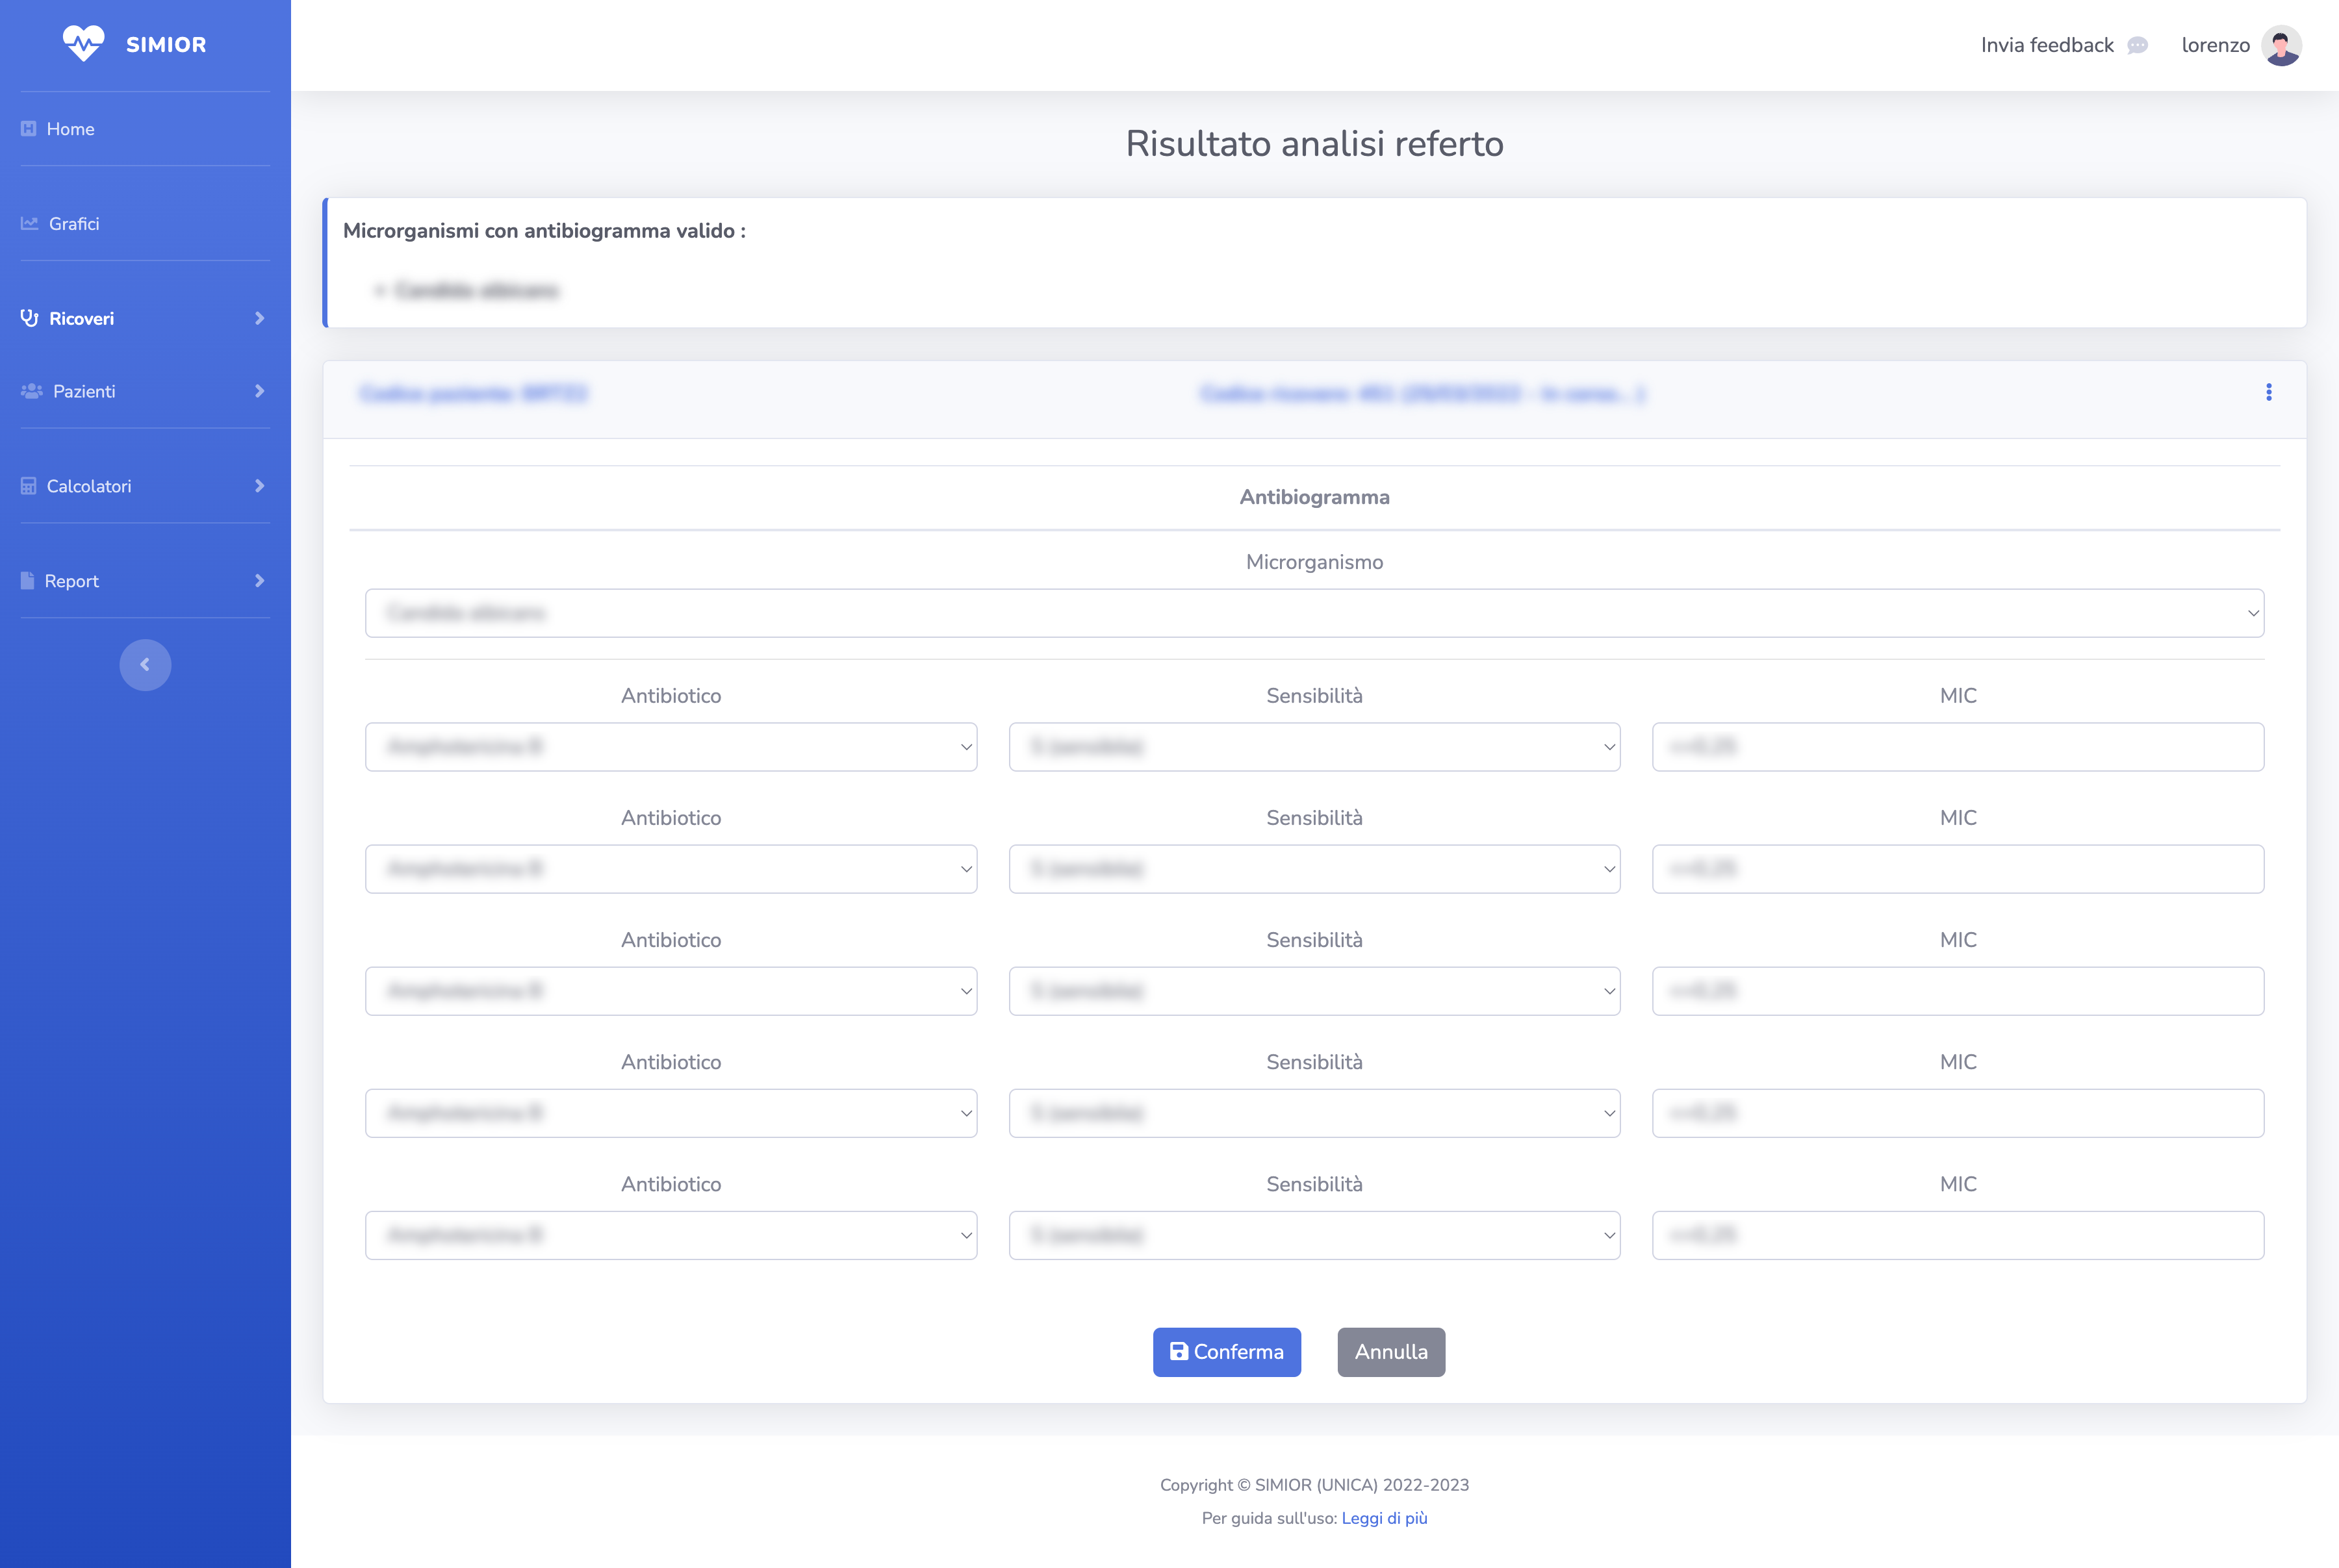
\includegraphics[width=.99\columnwidth]{images/extraction_result.png}
	\caption{\textit{Risultati estrazione}}
	\label{fig:extraction_result}
\end{figure}
\newline
Se un microrganismo non è presente nel sistema non è possibile inserire neanche il relativo antibiogramma perché non sarebbe poi possibile farvi riferimento successivamente.
\begin{figure}[h!]
	\centering
	
\includegraphics[width=.99\columnwidth]{images/static_missing.png}
	\caption{\textit{Microrganismo sconosciuto}}
	\label{fig:missing_micro}
\end{figure}
\newline
Allo stesso modo vengono segnalati eventuali antibiotici sconosciuti, ma a differenza del caso precedente, è comunque possibile procedere con l'inserimento dell'antibiogramma che verrà mostrato mancante dell'antibiotico relativo.
\begin{figure}[h!]
	\centering
	
\includegraphics[width=.99\columnwidth]{images/static_missing_antib.png}
	\caption{\textit{Antibiotico sconosciuto}}
	\label{fig:missing_anti}
\end{figure}
\newpage
In caso non tutti i dati siano estratti correttamente è possibile aggiungere o togliere manualmente informazioni, le opzioni di aggiunta sono disponibili nel menù drop-down posizionato in alto a destra nella scheda contenente la tabella.
Per modificare un valore errato è sufficiente scegliere un alternativa nella relativa lista, mentre per eliminare un valore (antibiotico o microrganismo) si seleziona l'elemento vuoto nella lista (indicato con un trattino), l'eliminazione ha un effetto 
"a cascata" che segue la seguente gerarchia: microrganismo -> antibiotico -> mic e sensibilità, quindi l'eliminazione dell'antibiotico elimina l'intera riga mentre l'eliminazione del microrganismo elimina l'intero antibiogramma associato
\begin{figure}[h!]
	\centering
	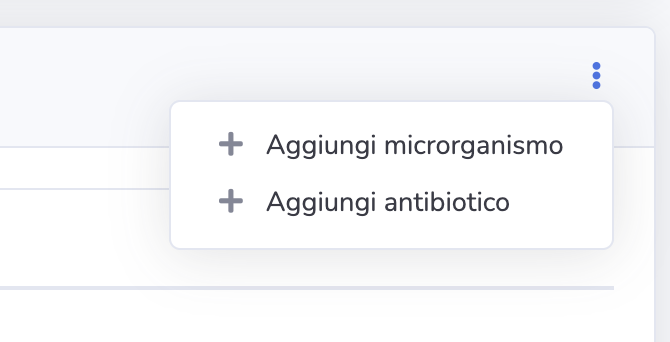
\includegraphics[width=.99\columnwidth]{images/new_object.png}
	\caption{\textit{Drop-down con le opzioni}}
	\label{fig:new_object}
\end{figure}